%********************************************************************
% Appendix
%*******************************************************
% If problems with the headers: get headings in appendix etc. right
%\markboth{\spacedlowsmallcaps{Appendix}}{\spacedlowsmallcaps{Appendix}}
\chapter{Calculation Details to Chapter 2}\label{app:A}

\section{Calculation of the spin-spin correlator} 
\label{app:spinspin}
%The spin polarization $\bb{s}_{\bb{q},\omega}$ needs to be averaged over many disorder realizations. In the Born approximation we replace each Green's function in Eq.~(\ref{chap1:eq:skubo}) with a disorder averaged one and replace one of the spin-operators with a vertex corrected spin operator. When calculating the components of $K_{\alpha\beta}$ that are of the order $\mathcal{O}(\ep\tau)^0)$, one should also include contributions from rare-scattering events. This is done by including the crossed diagrams depicted in Fig.~\ref{fig:diagrams}. 

%The disorder-averaged Green functions are obtained by including the Born self-energy $\Sigma^\text{R(A)}$ (we set $\hslash=1$ in the subsequent formulas)
\begin{equation}
  \im \Sigma^\text{R(A)} = 2\pi\alpha\, v^2 \im \int\!\frac{d^2\bb{p}}{(2\pi)^2}\left(\ep-H-\Sigma^\text{R(A)}\right)^{-1} = \mp \frac{\pi\alpha}{2} (\ep\sigma_0 -\Delta_z\sigma_3),
\end{equation}
The real part of $\Sigma^{\mathrm{R(A)}}$ lead to renormalization of $\ep$ and $\Delta_\textrm{sd}$. In the following we keep the same notation for $\ep$ and $\Delta_z$, though now they correspond to renormalized quantities. The Green functions are then given by
\begin{equation}
      G_{_\ep,\bb{p}}^{\mathrm{R(A)}} =
     \frac{
       \ep^\mathrm{R(A)}\sigma_0 + v\left(\bb{p}\times\bb{\sigma}\right)_z - \Delta_z^\mathrm{R(A)} \sigma_3}
       {(\ep^\text{R(A)})^2-v^2p^2-(\Delta_z^\text{R(A)})^2}
\end{equation}
where $\ep^{R(A)}=\ep(1\pm i\pi\alpha/2)$ and $\Delta_z^{R(A)}=\Delta_z(1\mp i\pi\alpha/2)$. The $\bb{m}_\para$ components were removed via the gauge transformation. 

Next, we need to replace the spin operator $\sigma_\alpha$ with a vertex corrected spin operator $\sigma_\alpha^\text{vc}$ in the ladder approximation as depicted in Fig.~\ref{fig:diagrams}(e). The dressing of $\sigma_\alpha$ with a single disorder line is denoted by $\sigma_\alpha^{1\times\text{dr}}$ and is defined by
    \begin{align}
       \sigma_\alpha^{1\times\text{dr}}  = 2\pi \alpha\, v^2 \int\!\frac{d^2\bb{p}}{(2\pi)^2} G^\text{A}_{\ep+\omega,\bb{p}+\bb{q}}\sigma_\alpha G^\text{R}_{\bb{p}} = \pi\alpha M_{\alpha\beta}\sigma_\beta,
        \label{chap1:eq:myseries}
    \end{align}
with $M_{\alpha\beta}=v^2\int\!d^2\bb{p}\tr\left[\sigma_\alpha G^\text{R}_{\ep+\omega,\bb{p}+\bb{q}}\sigma_\beta G^\text{A}_{\ep,\bb{p}}\right]/(2\pi)^2$. 
The ladder summation is conveniently represented in the matrix form by introducing a matrix $\hat{M}$ with $16$ components $M_{\alpha\beta}$ for $\alpha,\beta=0,x,y,z$ ($\sigma_0=1$). 

The crossed diagrams in Fig.~\ref{fig:diagrams} (b-d) give a contribution to the components of $\hat{K}$ of the order $\mathcal{O}(\alpha^0)$. The only components that are modified to this order are those corresponding to the Hall conductivity (i.e. $\alpha,\beta=1,2$ and vice versa). Details of this calculation can be found in Ref. \cite{ivan}. 

In our calculation the terms of the order of $\alpha \ln p_\textrm{cutoff}/\ep$ (where $p_\textrm{cutoff}$ is the ultraviolet momentum cut-off), is, therefore, disregarded with respect to $1$. This approximation is legitimate since we assume that all model parameters $\epsilon$, $\Delta_\textrm{sd}$ and $\alpha$ are first renormalized such that $p_\textrm{cutoff} \approx \ep$.

It is, then, easy to see that the vertex-corrected spin operator is readily obtained from the geometric series of powers of $\pi\alpha \hat{M}$, 
\begin{align}
\sigma_\alpha^\text{vc} &= 
\sigma_\alpha+\pi\alpha \hat{M}_{\alpha\beta}\sigma_\beta+(\pi\alpha)^2 (\hat{M}^2)_{\alpha\beta}\sigma_\beta+\dots\nonumber\\
&=\left[1-\pi\alpha \hat{M}\right]^{-1}_{\alpha\beta}\sigma_\beta,
\end{align}
where the summation of the repeating index $\beta=0,x,y,z$ is assumed. 

Thus, in the non-crossing approximation (illustrated in Fig.~\ref{fig:diagrams} (a)), one simply finds $\hat{K}= \hat{M}[1-\pi\alpha \hat{M}]^{-1}$. Dressed spin-spin correlators are defined by the components $ \hat{K}_{\alpha\beta}$ with $\alpha,\beta=x,y,z$. The matrix $\hat{M}$ will be computed to the second order in powers of $\omega$ and  $q$. 
%The result is represented as 

% \beml
% \label{chap1:eq:M}
% \begin{align}
% M &=M_0+M_\omega+M_{\omega^2}+M_{q\omega}+M_{q^2},\\
% M_0 &= 
% \frac{1}{\pi\alpha(\ep^2+\Delta_z^2)} 
% \bpm
% \ep^2& 0 & 0 & -\ep \Delta_z \\
%  0 & (\ep ^2-\Delta_z^2)/2 & \pi\alpha \ep \Delta_z & 0 \\
%  0 & -\pi \alpha \ep \Delta_z & (\ep ^2-\Delta_z^2)/2 & 0 \\
% -\ep \Delta_z & 0 & 0 & \Delta_z^2 
% \epm,\\
% M_\omega & =\frac{i\omega \ep}{\lt[\pi  \alpha  (\ep^2+\Delta_z^2)\rt]^2} 
% \bpm
% \ep^2 & 0 & 0 &-\ep\Delta_z\\
% 0 & (\ep ^2-\Delta_z^2)/2 & \pi \alpha (\ep^2-\Delta_z^2)\Delta_z/2\ep& 0 \\
%  0 &- \pi \alpha (\ep^2-\Delta_z^2)\Delta_z/2\ep& (\ep ^2-\Delta_z^2)/2  & 0 \\
% -\ep\Delta_z& 0 & 0 & \Delta_z^2  
% \epm,\\
% M_{\omega^2} & =\frac{(i\omega \ep)^2}{\lt[\pi  \alpha  (\ep^2+\Delta_z^2)\rt]^3}
% \bpm
% \ep^2 & 0 & 0 &-\ep\Delta_z\\
% 0 & (\ep ^2-\Delta_z^2)/2 & \pi \alpha (\ep^2-\Delta_z^2)\Delta_z/2\ep& 0 \\
%  0 & -\pi \alpha (\ep^2-\Delta_z^2)\Delta_z/2\ep& (\ep ^2-\Delta_z^2)/2  & 0 \\
% -\ep\Delta_z& 0 & 0 & \Delta_z^2  
% \epm,\\
% M_{q\omega} & =\frac{v(\ep^2-\Delta_z^2)}{\lt[\pi \alpha \left(\ep^2+\Delta_z^2\right)\rt]^2}\left(\frac{-i}{2}+ \frac{\ep\omega}{\lt[\pi\alpha(\ep^2+\Delta_z^2)\rt]}\right) 
% \bpm
%  0 & \ep  q_x& \ep  q_y& 0 \\
%  \ep  q_x & 0 & 0 & -\Delta_z q_x\\
%  \ep  q_y & 0 & 0 & -\Delta_z q_y\\
%  0 & -\Delta_z q_x & -\Delta_z q_y & 0 
% \epm,\\
% M_{q^2} & =\frac{v^2 (\ep^2-\Delta_z^2)}{2\lt[\pi\alpha(\ep^2+\Delta_z^2)\rt]^3} 
% \bpm
% \ep^2q^2& 0 & 0 & -\ep\Delta_z q^2 \\
%  0 & -(\ep^2-\Delta_z^2) (3q_x^2-q_y^2)/4 & - (\ep^2-\Delta_z^2) q_xq_y/2 & 0 \\
%  0 & - (\ep^2-\Delta_z^2) q_xq_y/2 & -(\ep^2-\Delta_z^2) (3q_y^2-q_x^2)/4 & 0 \\
% -\ep \Delta_z q^2  & 0 & 0 & \Delta_z^2q^2
% \epm,
% \end{align}
% \eml

% from which the components of $\hat{K}$ are obtained. 
%Using the result for $M$ we, then, compute the tensor $\hat{K}$ as
%\begin{equation}
%\hat{K}_{}=
%  \begin{pmatrix}
% \sigma_{xx} & \sigma_{xy} & Q_y \\ \sigma_{yx} & \sigma_{yy} & -Q_x \\ Q_y & -Q_x & \zeta
%  \end{pmatrix}.
%\end{equation}
Complete expressions for the components are cumbersome, therefore we proceed by first analyzing their denominator, which is proportional to $\det [1-\pi\alpha M]$

\begin{multline}
  \det [1-\pi\alpha M]=
   -\frac{\varepsilon  \left(\varepsilon ^2+3\Delta_z^2\right)^2}{4 \pi  \alpha  \left(\varepsilon ^2+\Delta_z^2\right)^3}\times\left(i\omega\left(1-i\omega\tau_\text{tr}\frac{\varepsilon^2-5\Delta_z^2}{\varepsilon^2-\Delta_z^2}+\mathcal{O}((\omega\tau_\text{tr})^2)\right)\right.%\nonumber
   \\
   \left.-Dq^2\left(1+i\omega\tau_\text{tr}\frac{13\Delta_z^4+10\Delta_z^2\varepsilon^2+\varepsilon^4}{(\varepsilon^2-\Delta_z^2)(\varepsilon^2+\Delta_z^2)}-(i\omega\tau_\text{tr})^2\frac{(\varepsilon^2+3\Delta^2)(\varepsilon^4-14\varepsilon^2\Delta_z-35\Delta_z^4)}{(\varepsilon^2-\Delta_z^2)(\varepsilon^2+\Delta_z^2)}\right.\\
   \left.+\mathcal{O}((\omega\tau_\text{tr})^3)\right)+\mathcal{O}((Dq^2)^2\tau_\text{tr})\right).
   %
\label{chap1:eq:sdet}
\end{multline}

By restricting ourselves to perturbations that vary slow in time compared to the transport time $\tau_\text{tr}$ and smooth in space compared to the diffusion length $L_D=\sqrt{D\tau_\text{tr}}$, i.e. $\omega\tau_\text{tr},Dq^2\tau_\text{tr}\ll1$, we are able to extract the diffusion pole $(i\omega-Dq^2)^{-1}$.

The components of the conductivity tensor $\hat{\sigma}$ at finite $\omega$ and $\bb{q}$ are given by
\beml
\label{chap1:eq:sconductivity}
\begin{align}
  \sigma_{xx} &= \sigma_0+\frac{Dq^2}{i\omega-Dq^2}\left(\frac{q_y^2}{q^2} \sigma_0
  -i\omega \tau_\text{tr}\left(\frac{2}{\pi\alpha}\frac{\varepsilon^2+2\Delta_z^2}{\varepsilon^2+\Delta_z^2}+\frac{3}{\pi\alpha}\frac{q_{x}^2-q_{y}^2}{2q^2}\right)\right)\\
  %
  \sigma_{yy} &=  \sigma_0+\frac{Dq^2}{i\omega-Dq^2}\left(\frac{q_x^2}{q^2} \sigma_0
    -i\omega \tau_\text{tr}\left(\frac{2}{\pi\alpha}\frac{\varepsilon^2+2\Delta_z^2}{\varepsilon^2+\Delta_z^2}-\frac{3}{\pi\alpha}\frac{q_{x}^2-q_{y}^2}{2q^2}\right)\right)\\
    %
    \sigma_{xy} &= \sigma_\textrm{H}+\frac{Dq^2}{i\omega-Dq^2}\left(-\frac{q_xq_y}{q^2} \sigma_0-i\omega\tau_\text{tr}\frac{3}{\pi\alpha}\frac{q_xq_y}{q^2}\right)\\
    %
  \sigma_{yx} &= -\sigma_\textrm{H}+\frac{Dq^2}{i\omega-Dq^2}\left(-\frac{q_xq_y}{q^2} \sigma_0-i\omega\tau_\text{tr}\frac{3}{\pi\alpha}\frac{q_xq_y}{q^2}\right),
\end{align}
\eml
where $\sigma_0$ and $\sigma_\textrm{H}$ are given in Eq.~(\ref{cond}) of the main text. 
The remaining components of $\hat{K}$ are given by
\beml
\label{Qresult}
\begin{align}
&\bb{Q}=\frac{\Delta_z}{ v}\, \frac{i D \bb{q}}{i\omega-Dq^2}
\lt(1+i\omega\tau_\text{tr}\frac{(\varepsilon^2+7\Delta_z^2)}{\varepsilon^2+\Delta_z^2}\rt),\\
&\zeta=\frac{\Delta_z^2}{ \ep}\,\frac{1-i\omega\tau_\text{tr}(\varepsilon^2-5\Delta_z^2)/(\varepsilon^2-\Delta_z^2)}{i\omega-Dq^2+\omega^2\tau_\text{tr}(\varepsilon^2-5\Delta_z^2)/(\varepsilon^2-\Delta_z^2)}
,
\end{align}
\eml
 where the $\omega^2$-term was included in the denominator of $\zeta$ because of its importance when taking the limit $q\rightarrow 0$.
%\begin{equation}
%\lim_{q\rightarrow 0}\zeta=\frac{\Delta_z^2}{2 \ep}\,\left(\frac{1}{i\omega}-\frac{\varepsilon}{\pi\alpha(\epsilon^2+\Delta_z^2)}\right).
%\label{chap1:eq:sszz}
%\end{equation}
The leading contributions to Eq.~(\ref{Qresult}a) in the limit $\omega\tau_\text{tr}\ll 1$ together with Eq.~(\ref{Qresult}b) in the limit $q\rightarrow0$ corresponds to Eqs.~(\ref{Kten},\ref{cond},\ref{szz}) of the main text. 

It is convenient to rotate the coordinate system such that the new $\hat{\bb{x}}$ axis lies along $\bb{q}$. Let us introduce a rotation matrix $U$ to transform the tensor $\hat{K}$,  
\begin{equation}
    U = \begin{pmatrix}
            q_x/q & -q_y/q & 0 \\
            q_y/q & q_x/q &0 \\
            0 & 0 & 1
        \end{pmatrix},\hspace{1cm}
    \tilde{K} = U^\top \hat{K} U,
\end{equation}
so that the new components of Eqs.~(\ref{chap1:eq:sconductivity}) become
\beml
\label{chap1:eq:sconductivity2}
\begin{align}
  \tilde{\sigma}_{xx} &= \sigma_0-\frac{Dq^2}{i\omega-Dq^2}i\omega \tau_\text{tr}\frac{7\varepsilon^2+11\Delta_z^2}{2\pi\alpha (\varepsilon^2+\Delta_z^2)}\\
  \tilde{\sigma}_{yy} &= \sigma_0+\frac{Dq^2}{i\omega-Dq^2} \left(\sigma_0-i\omega \tau_\text{tr}\frac{\varepsilon^2+5\Delta_z^2}{2\pi\alpha(\varepsilon^2+\Delta_z^2)}\right)\\
    \tilde{\sigma}_{yx} &= -\tilde{\sigma}_{xy}=\sigma_\textrm{H},
\end{align}
\eml
and the rotated, $\tilde{K}$, tensor is conveniently written as
\begin{equation}
    \tilde{K} = \begin{pmatrix} \tilde{\sigma}_{xx}         & \sigma_\textrm{H} & 0 \\
                                -\sigma_\textrm{H}  & \tilde{\sigma}_{yy}       & Q \\
                                0                   & Q                 & \zeta
                \end{pmatrix}.
\end{equation}

\section{Limiting behavior of m(t)}\label{app:A:lim}
%The equation of motion for the magnetization direction $\bb{m}$ reads
%\begin{equation}
%\label{eom}
%    \frac{\partial\bb{m}}{\partial t} = - \gamma\,\bb{m}\times\bb{H}_\text{eff} + f(\bb{r},t)\,\bb{m}\times\bb{m}_\perp+\alpha_\textrm{G}\, \bb{m}\times\frac{\partial\bb{m}_\para}{\partial t},
%\end{equation}
%where $\gamma$ is a gyromagnetic ratio, $\bb{H}_\text{eff}$ is an external effective field,  $\alpha_\textrm{G}=J_\text{sd}^2\mathcal{A}S\sigma_0/\pi(\hslash v)^2$ is a Gilbert damping (which is independent of energy for $\varepsilon\gg\Delta_\text{sd}$) and the function $f(\bb{r},t)$ is given by
%\begin{equation}
%  f(\bb{r},t) = -\eta \int\!\mathrm{d}^2\bb{r}'\int_{-\infty}^t\!\mathrm{d}t\,\frac{e^{-(\bb{r}-\bb{r}')^2/4D(t-t')}}{4\pi(t-t')}\bb{\nabla}\cdot\bb{E}(\bb{r}',t').
%\end{equation}
%The function $f(\bb{r},t)$ defines space and time dependence of the diffusive spin-torque. 
%
%%%
% Fig. 4
%%%
%$\begin{figure}[bt]
%\centering
%\centerline{\hspace*{1cm}\includegraphics[width=0.5\linewidth]{{fig2}}}
%\caption{The projection $m_\textrm{H}(t)$ as simulated from Eq.~(\ref{equation}) for $f_0=0.1\, \omega_0$.  
%Top panel illustrates the behavior at different frequencies for $\alpha_\textrm{G}=0.005$. Lower panel illustrates the resonant behavior at different values of $\alpha_\textrm{G}$. Dashed horizontal line corresponds to $m_\textrm{H}=1/\sqrt{2}$. Dots indicate the asymptotic solution for $\alpha_\textrm{G}=0$ as given by Eq.~(\ref{asymptot}).}
%\label{snum}
%\end{figure}

To illustrate the behavior of $\bb{m}(t)$ we consider $f=f_0\,\cos(\omega t)$ at a particular point $\bb{r}$. It is, also, convenient to let the field $\bb{H}_\mathrm{eff}$ to lie in the $\hat{\bb{x}}-\hat{\bb{z}}$-plane and rotate the coordinate system such that $\bb{H}_\mathrm{eff}$ lies along new z-direction. This is achieved by introducing the rotation matrix $\hat{R}$,  
\begin{align}
    \hat{R} = \begin{pmatrix} \cos\chi & 0 & -\sin \chi \\ 0 & 1 & 0 \\ \sin\chi & 0 & \cos\chi\end{pmatrix},
\end{align}
where $\chi$ is the angle between $\hat{\bb{z}}$ and $\bb{H}_\mathrm{eff}$. Furthermore, introducing the frequency $\omega_0 = |\gamma\bb{H}_\mathrm{eff}|$ and the unit vector $\bar{\bb{h}}=(-\sin\chi,0,\cos\chi)^\top$, we can write the equation of motion in the rotated coordinate frame as
\begin{multline}
    \partial_t \bb{m} = -\omega_0\,\bb{m}\times \hat{\bb{z}}+f(\bb{r},t)\,\lt(\bb{m}\cdot\bar{\bb{h}}\rt)\;\lt[\bb{m}\times\bar{\bb{h}}\rt]
    \\+
    \alpha_\textrm{G}\, \lt[\bb{m}\times (\partial_t\bb{m})\rt]
    -\alpha_\textrm{G}\, (\partial_t \bb{m})\cdot \hat{\bb{z}}\;\lt[\bb{m}\times \hat{\bb{z}}\rt],
    \label{dynamicEQ}
\end{multline}
where the vector $\hat{\bb{z}}$ is defined now as the unit vector along $\bb{H}_\mathrm{eff}$, hence the magnetization projection $m_\text{H}=\bb{m}\cdot\bb{h}$ is simply given by $m_z$. 

%The numerical solution of Eq.~(\ref{dynamicEQ}) for the time evolution of $m_\text{H}$ is illustrated in Figs.~\ref{fig:dynamics},\ref{fig:sbloch} assuming the initial condition $m_H=0.9999$ at $t=0$. In Fig.~\ref{fig:sbloch} we plot the Bloch trajectory of the spin for different parameter choices. 

%%%
% Fig. 5
%%%
%\begin{figure}[bt]
%    \centering
%    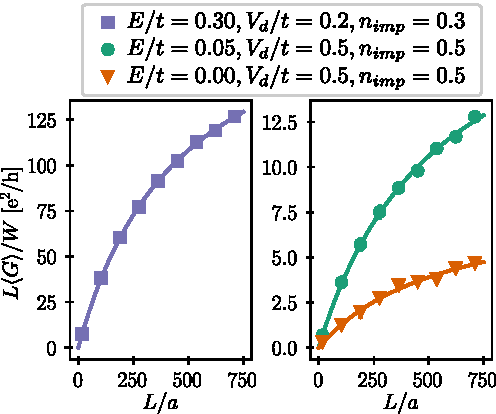
\includegraphics[width=0.95\columnwidth]{fig4}
%    \caption{Real-space visualization of the trajectory of $\bb{m}$ at different driving frequencies $\omega$, corresponding to the top panel in Fig.~\ref{fig:dynamics}}
%    \label{fig:sbloch}
%\end{figure}

In the regime of $\alpha_\textrm{G}\ll f_0 \ll \ll \omega_0$ we can find the asymptotic behavior of $m_\textrm{H}$ at sufficiently small times. In order to do that it is convenient to represnt $\bb{m}$ in spherical coordinates: $\bb{m}=(\sin\theta\cos\phi,\sin\theta\sin\phi,\cos\theta)^\top$, where $\theta$ is the polar angle between $\bb{m}$ and $\hat{\bb{z}}$ and $\phi$ is the azimuth. In the limit $\alpha_\textrm{G}\rightarrow 0$ we find the equations of motion on $\theta$ and $\phi$:
\begin{align}
\partial_t \theta &= \sin \chi  \sin \phi  f(\bb{r},t) \big(\sin \chi  \sin \theta \cos \phi -\cos \chi  \cos \theta \big)\\
\partial_t \phi &=\omega_0+f(r,t) 
  \cos\theta\big(\cos ^2\chi  \cos ^2\phi-\sin^2\phi -\frac{1}{2}\sin\chi(\cot\theta-\sin\theta) \big).
\end{align}
We take $f(\bb{r},t)=f_0\cos\omega t$ and assume that $f_0\ll\omega_0$, so that we find $\phi = \omega_0 t-\phi_0$. It is convenient to choose $\phi_0=\pi/2$ so that
\begin{align}
  \partial_t \theta = -f_0 \sin \chi  \cos ^2\omega_0t\,(\sin \theta  \sin \chi  \sin \omega_0t-\cos \theta  \cos \chi ).
  \label{chap1:eq:theta2}
\end{align}
Because we assumed that $f_0\ll\omega_0$, the dynamics of $\phi$ is much faster than the dynamics of $\theta$. Therefore we average Eq.~(\ref{chap1:eq:theta2}) over $\phi$ and obtain
\begin{equation}
  \partial_t\theta = \frac{f_0}{4} \cos \theta \sin2\chi.
\end{equation}
This equation is readily solved by means of the substitution $\cos\theta = 1/\cosh x$, $\sin\theta=-\tanh x$. Using the initial condition $\theta(0)=0$ one finds 
\begin{equation}
\cos\theta(t) = \frac{1}{\cosh\lt( \frac{1}{4}f_0 t \sin2\chi\rt)},
\end{equation}
which gives the result of Eq.~(\ref{asymptot}) of the main text.

